%
\documentclass[12pt]{article}
\usepackage{times}
\usepackage{amssymb}
\usepackage{amsmath}
\usepackage{url}
\setlength{\topmargin}{-5mm} \setlength{\evensidemargin}{-6mm}
\setlength{\oddsidemargin}{-6mm} \setlength{\textwidth}{162mm}
\setlength{\textheight}{230mm} \setlength{\parskip}{1.0ex}
\setlength{\parindent}{0pt}
%\bibliographystyle{unsrt}
\usepackage{graphicx}

\begin{document}

\newcommand{\Hide}[1]{}
\begin{center}
{\LARGE \bf A flexible structured service composition based on runtime construction of synergistic      elementary service groups}\\

\end{center}

{\bf Abstract}: the contribution of this paper is to: 1) proposed a general structure for component services which allows flexible constructing component service in runtime. 2) formulated a more general QoS-aware service composition problem by relaxing the one-to-one mapping between subtasks  and atomic services. 3) provided a  solution based on SMT solver.  \\
{\bf Keywords}: service composition, runtime constructed component service; quality of service (QoS)
\section*{Introduction}
\section*{Motivated example}
In order to illustrate the issue addressed in this work, an example about ��online motorcycle production (OMP)�� is presented in the context of CMfg. The flow of OMP is shown in Fig.\ref{OMP}, where six key sections (subtasks) are considered.

\begin{figure}[htbp]
\centering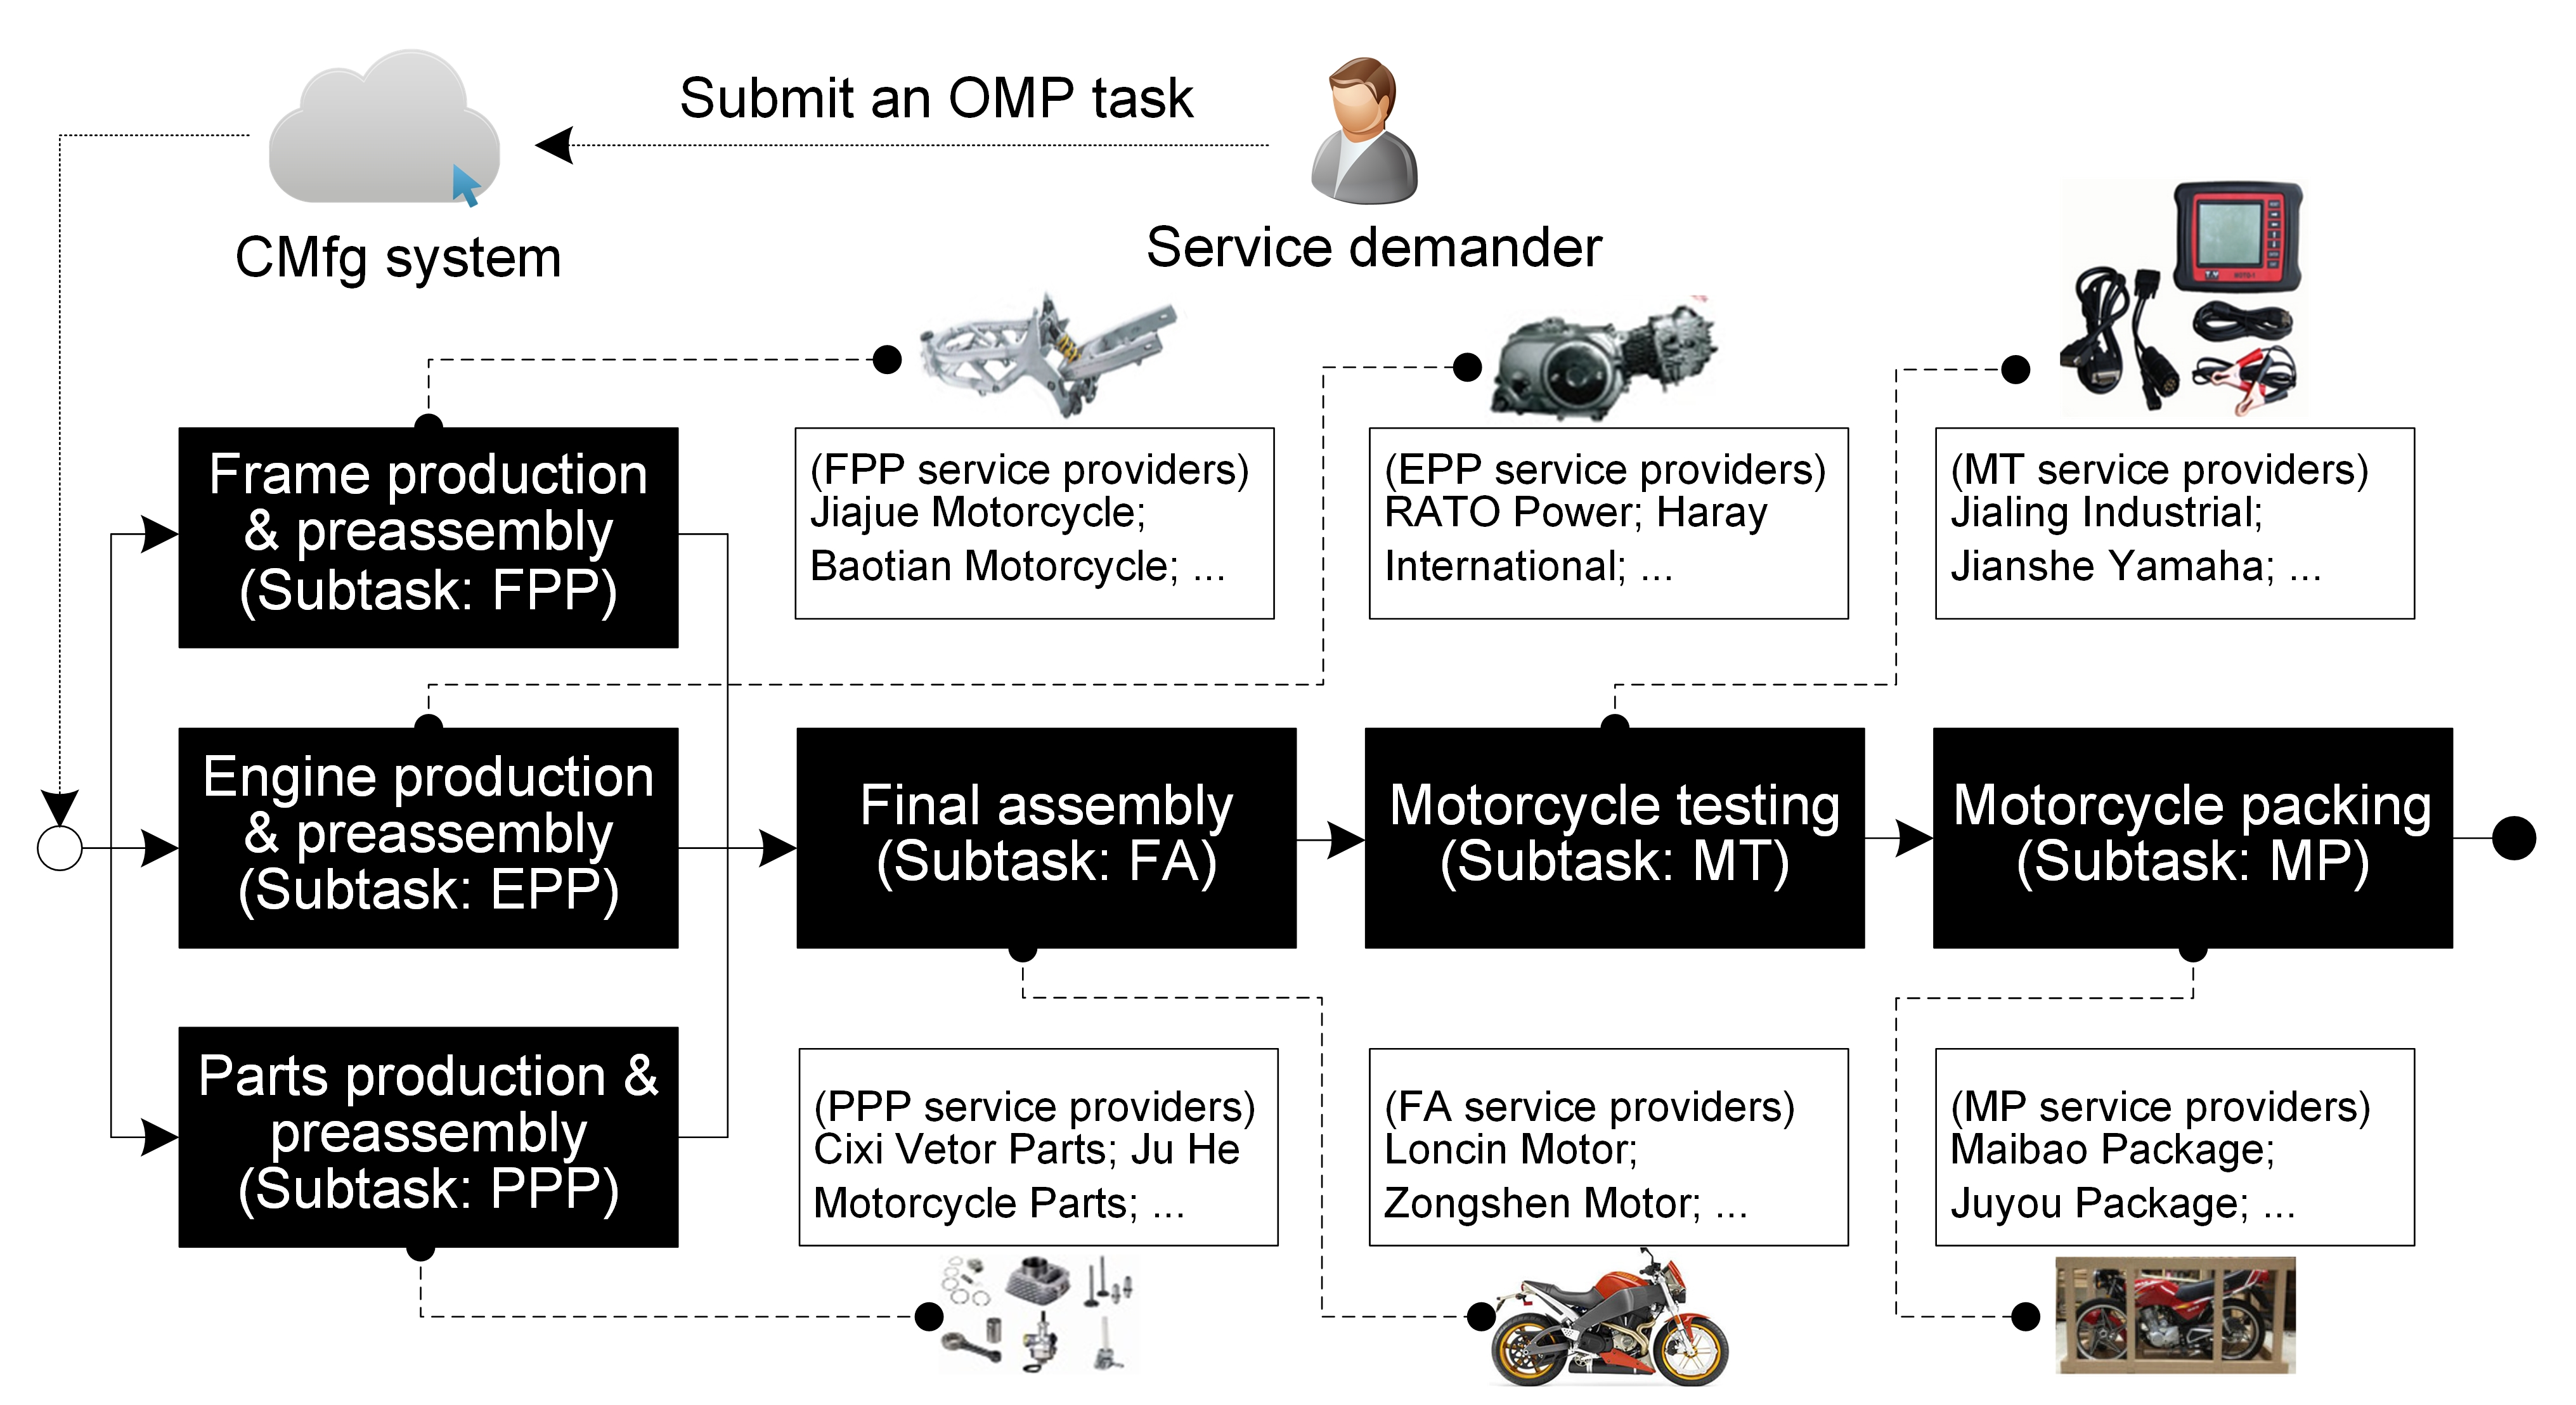
\includegraphics[scale=0.8]{figs/Fig1.jpg}
\caption{Workflow of online motorcycle production (OMP)
\label{OMP}}
\end{figure}

\section*{Formulation of the problem}

We improve the model of QoS-aware service composition by using synergistic elementary service groups (\textit{SESGs}) as the elementary services, instead of using atomic services directly(as shown in Fig.\ref{SESG_SC_fig}).

\begin{figure}[htbp]
\centering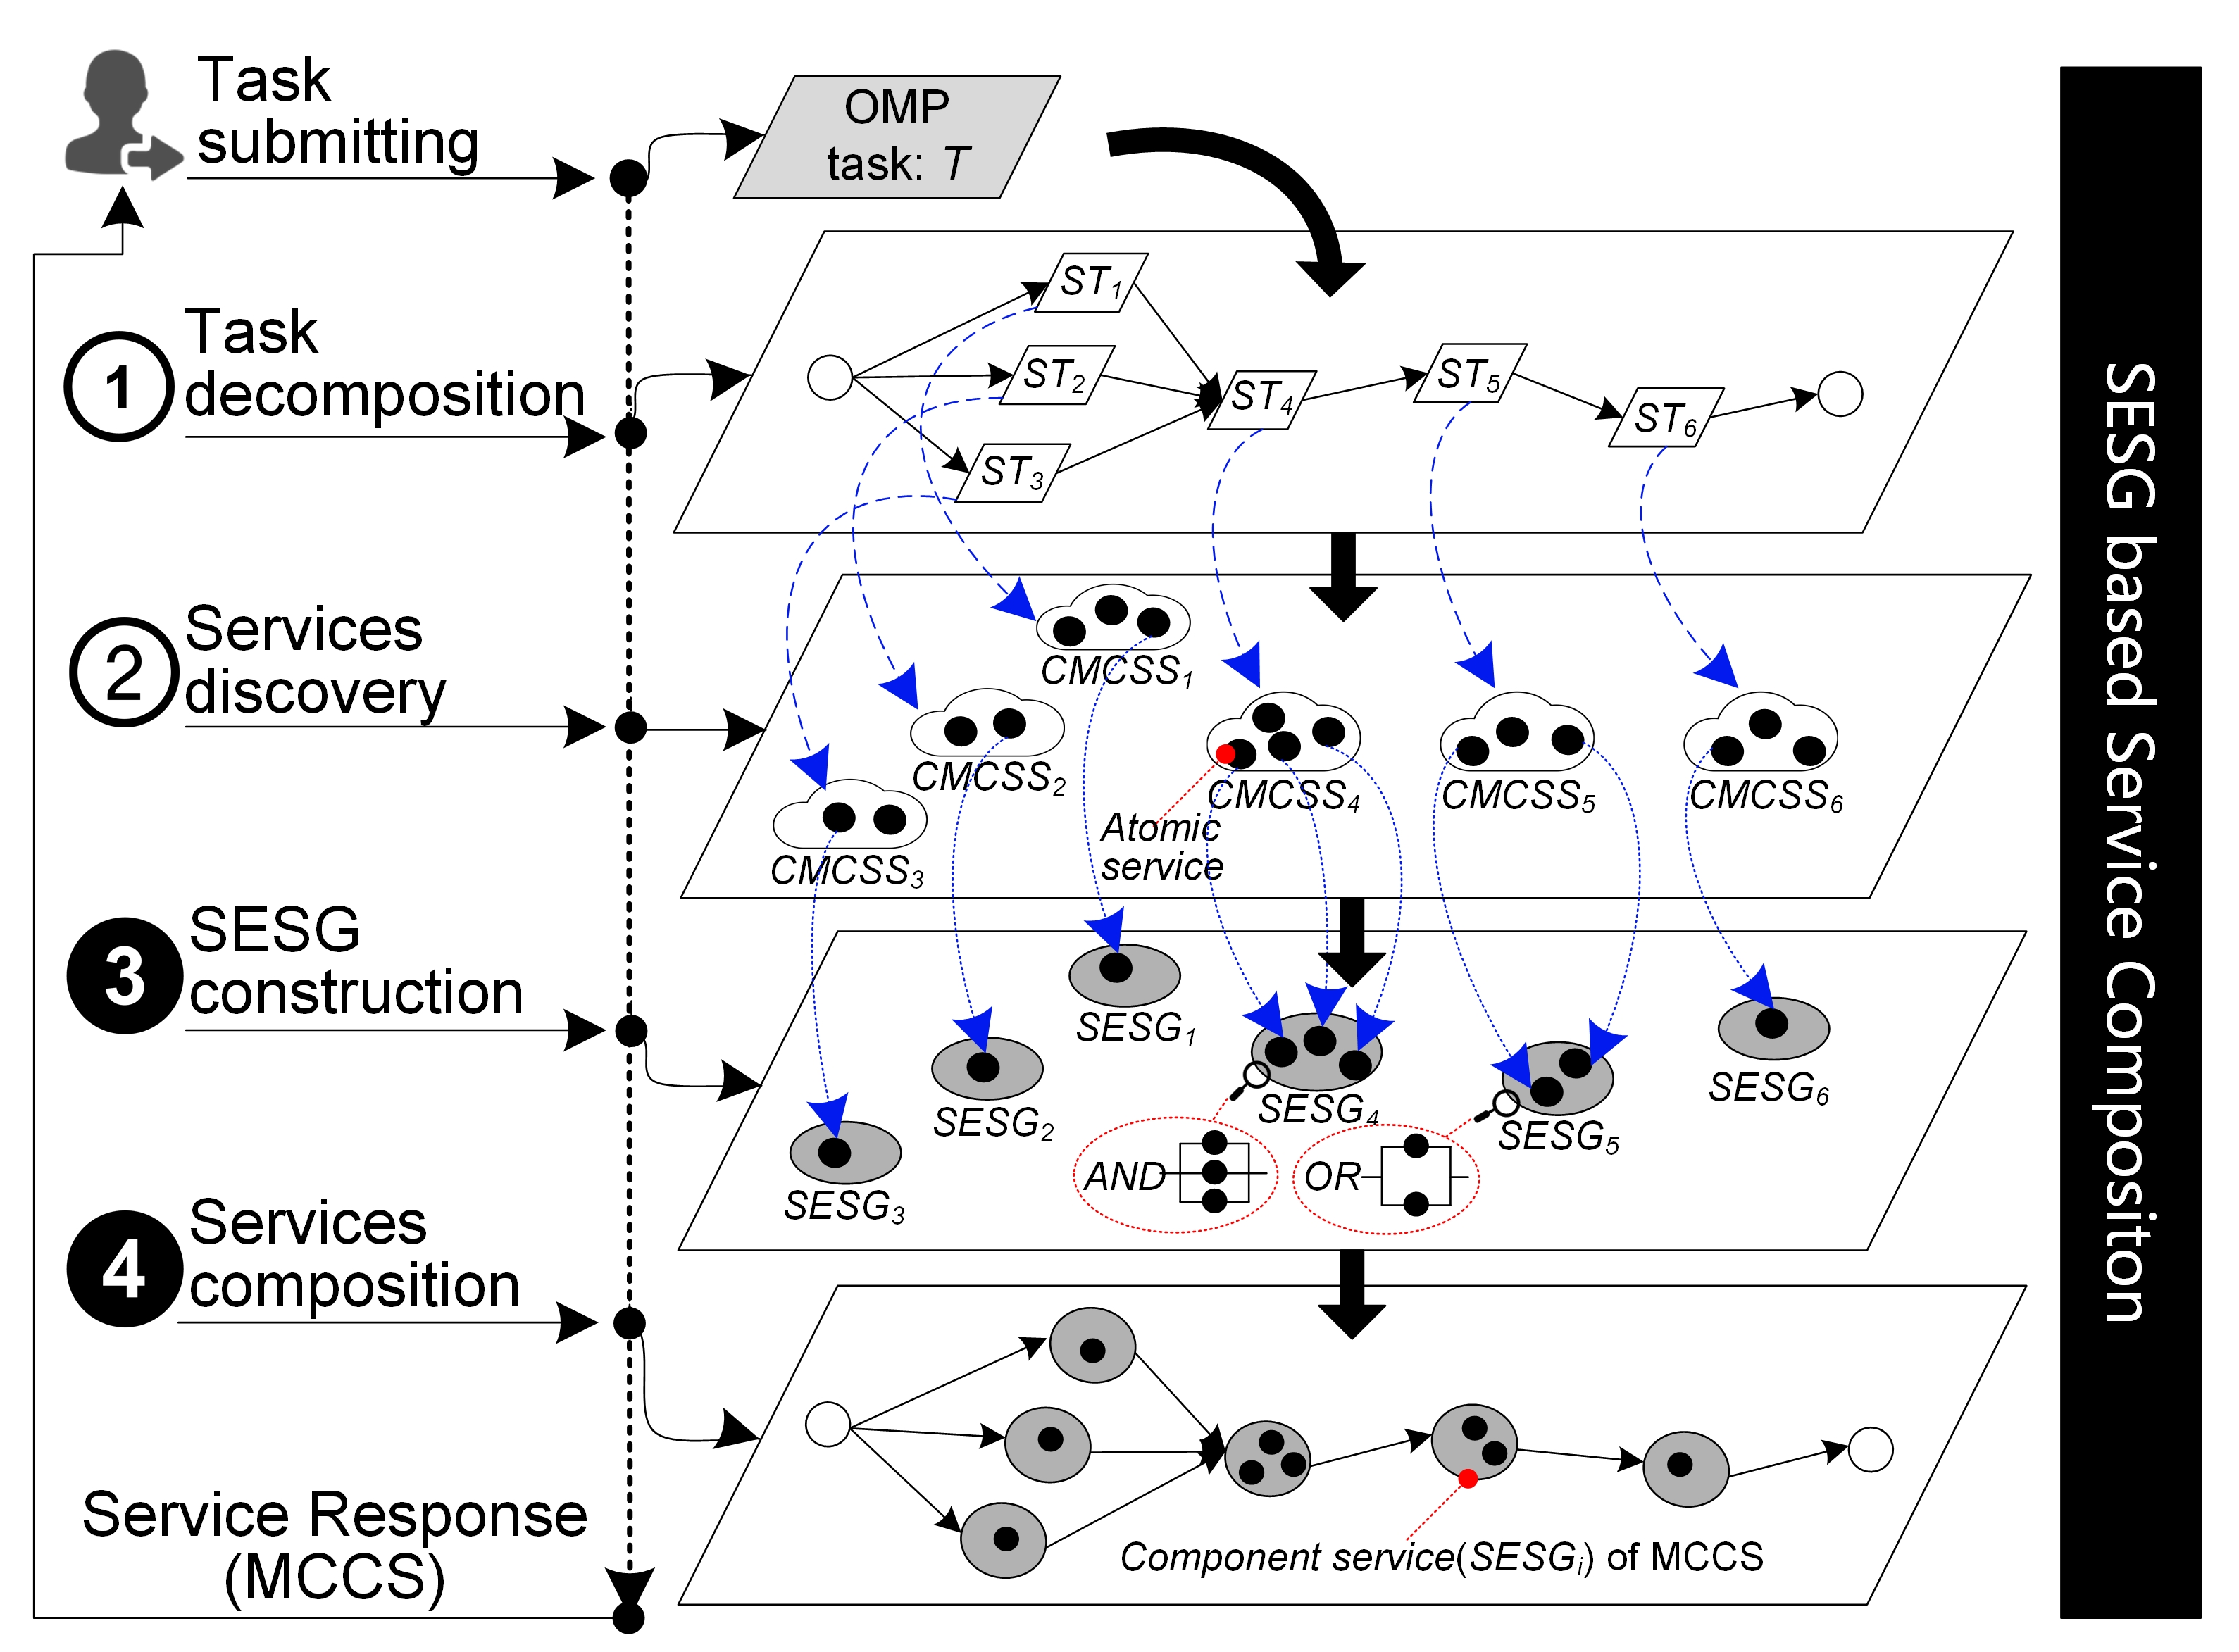
\includegraphics[scale=0.8]{figs/Fig2.jpg}
\caption{SESGs based service composition
\label{SESG_SC_fig}}
\end{figure}

A \textit{SESG} is a general elementary service for flexible structured QoS-aware service composition. As shown in Fig.\ref{SESGfig}, each \textit{SESG} contains two parts: 1) the parallel structure, and 2) the selective structure. These two parts are both dynamically constructed with the runtime selected atomic services, and the two parts are bound together in a parallel mode.

\begin{figure}[htbp]
\centering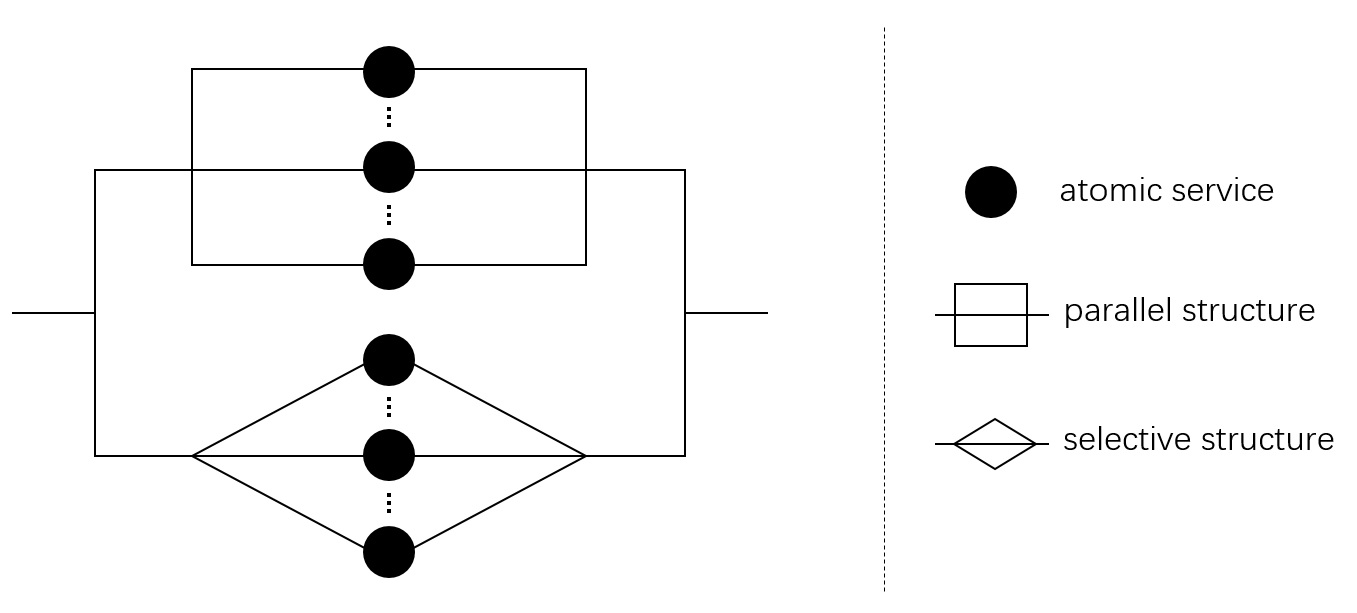
\includegraphics[scale=0.8]{figs/Fig3.jpg}
\caption{a general elementary service with runtime binding atomic services
\label{SESGfig}}
\end{figure}

Let $s_{ij}$ denotes the $j$-th candidate atomic service that could be selected into the $SESG_{i}$ for a subtask $ST_{i}$ , where $i \in[1,I]$, $j \in[1,J]$;   the constant $I$ and $J$ denote the numbers of subtasks and atomic services, respectively.

Let $x_{ij} = 1$ denotes the $j$-th atomic service is chosen into the parallel part of $SESG_{i}$, otherwise, $ x_{ij} = 0$; Let $ y_{ij} = 1$ denotes the $j$-th atomic service is chosen into the selective part of $SESG_{i}$, otherwise, $ y_{ij} = 0$; such that:

\begin{equation}
\label{not_both_selected}
\neg (x_{ij} = 1\wedge y_{ij} = 1)
\end{equation}

\begin{equation}
\label{constrain_on_total_number}
\sum_{j=1}^{J}x_{ij}+\sum_{j=1}^{J}y_{ij}\geq1
\end{equation}

Eq.\ref{not_both_selected} indicates one atomic service can  be chosen into either the parallel or selective part of $SESG_{i}$, or not to be chosen; the case that one atomic service is selected into both two parts is not allowed. Eq.\ref{constrain_on_total_number} indicates that at least one atomic service will be chosen into either the parallel or selective part of $ SESG_{i}$.

Let $T(\cdot)$, $C(\cdot)$, $R(\cdot)$ denotes the time, cost, and reliability property of QoS, respectively. Then, the formulas to calculate the QoS of $SESG_{i}$ are as follows:

\begin{equation}
\label{SESG_cost}
C(SESG_{i})=\underbrace{\sum_{j=1}^{J}C(s_{ij})\times x_{ij}}_{cost\ of\ the\ parallel\ part}+\underbrace{\sum_{j=1}^{J}C(s_{ij})\times p_{ij}}_{cost\ of\ the\ selective\ part}
\end{equation}

\begin{equation}
\label{SESG_time}
T(SESG_{i})=\frac{1}{\underbrace{\sum_{j=1}^{J}\frac {1}{T(s_{ij})}\times x_{ij}}_{work\ efficiency\ of\ the\ parallel\ part}+\underbrace{\sum_{j=1}^{J}\frac{1}{T(s_{ij})}\times p_{ij}}_{work\ efficiency\ of\ the\ selective\ part}}
\end{equation}

\begin{equation}
\label{SESG_reli}
R(SESG_{i})=\underbrace{(\prod_{j=1}^{J}R(s_{ij})^ {x_{ij}})^{sgn(\sum_{j=1}^{J} x_{ij})}}_{reliability\ of\ the\ parallel\ part}\times \underbrace{R(sel(SESG_{i}))}_{reliability\ of\ the\ selective\ part}
\end{equation}

where the reliability of the selective part of $SESG_{i}$ can be defined as follows:

\begin{equation}
\label{SESG_reli_sel}
\begin{aligned}
((\sum_{j=1}^{J} y_{ij}>0)&\Rightarrow (R(sel(SESG_{i})=\sum_{j=1}^{J}R(s_{ij})^{y_{ij}} \times {p_{ij}}))\quad \wedge \\ ((\sum_{j=1}^{J} y_{ij}=0)&\Rightarrow (R(sel(SESG_{i}))=1))
\end{aligned}
\end{equation}


The variable $p_{ij}$ in Eq.\ref{SESG_time} - \ref{SESG_reli_sel} denotes the probability of the selected atomic service $s_{ij}$ within the selective part of $SESG_{i}$ to undertake the subtask $ST_{i}$. We assume that the probability of $s_{ij}$ is related to the reliability of $s_{ij}$; because in many real cases, the service of higher reliability is more likely to get the chance to undertake a task, when   a group of services  compete with each other in a selective mode. On account of this assumption, we express  $p_{ij}$ as follows:

\begin{equation}
\label{pij}
((\sum_{j=1}^{J} y_{ij} \geq1)\Rightarrow(p_{ij}=\frac{R(s_{ij})\times y_{ij}}{\sum_{j=1}^{J} R(s_{ij})\times y_{ij}}))\wedge((\sum_{j=1}^{J} y_{ij} <1)\Rightarrow(p_{ij}=0))
\end{equation}

Eq.\ref{pij} indicates that if at least one atomic service is chosen into the selective part of $SESG_{i}$, the probability of $s_{ij}$ can be calculated according to the proportion of its reliability in the accumulated reliability of all chosen atomic services; otherwise, the probability equals zero.

Till now, the formulas of the time, cost and reliability property of QoS have been defined for a general elementary component service $SESG_{i}$ in \textit{SESG}s based service composition. By using the aggregation formulas in traditional QoS-aware service composition (as shown in Fig.\ref{Agg_formulas}), the QoS evaluation of the overall workflow of OMP can be performed.

\begin{figure}[htbp]
\centering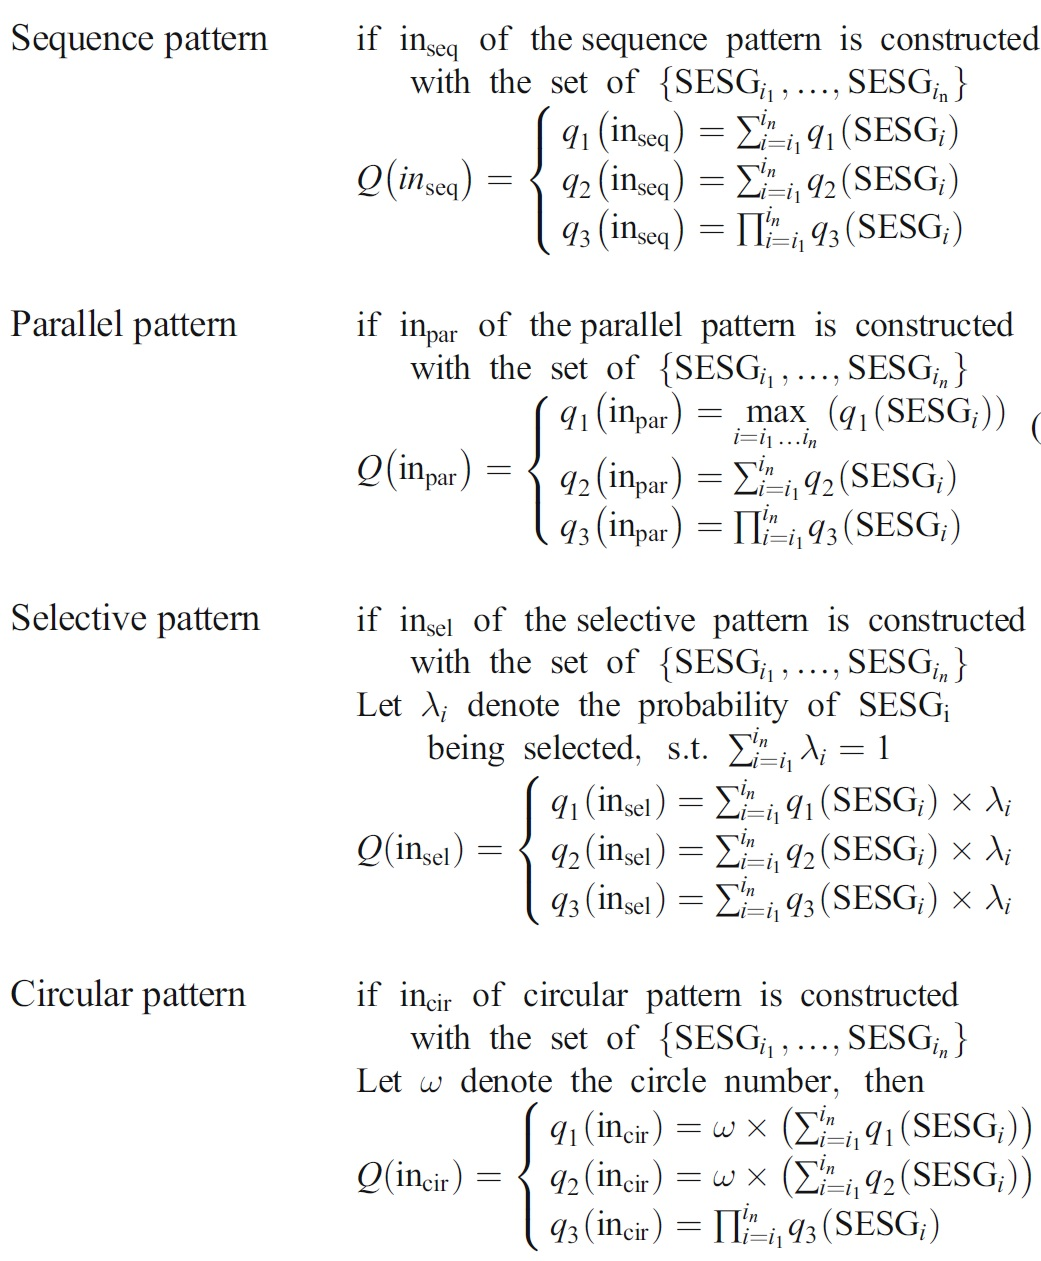
\includegraphics[scale=0.8]{figs/Fig4.jpg}
\caption{Aggregation formulas to evaluate workflow fragments of different patterns
\label{Agg_formulas}}
\end{figure}

As shown in Fig. \ref{OMP}, the workflow of OMP involves six subtasks. The first three subtasks are parallel, and the last three are sequential. Since the QoS properties of time, cost and reliability for each atomic service are given, the QoS value of a general elementary service $SESG_{i}$ for a given subtask $ST_{i}$ can be calculated based on Eq. \ref{SESG_cost} - \ref{pij}. Then, the QoS value of a possible composite service (\textit{CS}) for the OMP task can be calculated as follows:

\begin{subequations}
\begin{align}
T(CS) &= max(T(SESG_{1}),T(SESG_{2}),T(SESG_{3}))+ \sum_{i=4}^{6}T(SESG_{i}) \\
C(CS) &= \sum_{i=1}^{6}C(SESG_{i}) \\
R(CS) &= \prod_{i=1}^{6}R(SESG_{i})
\end{align}
\end{subequations}

A simple additive weighting (SAW) technique is used to deal with the different magnitudes of QoS properties and obtain a score from diverse QoS dimensions.Positive and negative properties are scaled in different ways, as defined in Eqs. and , respectively.

\begin{subequations}
\begin{align}
\begin{split}
\left\{
\begin{aligned}
(max(T(\cdot))= min(T(\cdot)) &\Rightarrow \overline{T}(\cdot)=1) \wedge \\
(max(T(\cdot))\not= min(T(\cdot))&\Rightarrow \overline{T}(\cdot)=\frac{max(T(\cdot))-T(\cdot)}{max(T(\cdot))-min(T(\cdot))}))
\end{aligned}
\right.
\end{split} \\
\begin{split}
\left\{
\begin{aligned}
(max(C(\cdot))= min(C(\cdot)) &\Rightarrow \overline{C}(\cdot)=1) \wedge \\
(max(C(\cdot))\not= min(C(\cdot))&\Rightarrow \overline{C}(\cdot)=\frac{max(C(\cdot))-C(\cdot)}{max(C(\cdot))-min(C(\cdot))}))
\end{aligned}
\right.
\end{split} \\
\begin{split}
\left\{
\begin{aligned}
(max(R(\cdot))= min(R(\cdot)) &\Rightarrow \overline{R}(\cdot)=1) \wedge \\
(max(R(\cdot))\not= min(R(\cdot))&\Rightarrow \overline{R}(\cdot)=\frac{C(\cdot)-min(C(\cdot))}{max(C(\cdot))-min(C(\cdot))}))
\end{aligned}
\right.
\end{split} 
\end{align}
\end{subequations}


\end{document}
